\begin{XeClass}{Options}
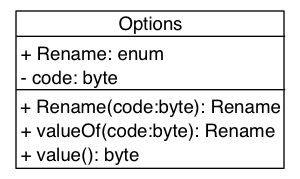
\includegraphics[width=10cm]{cdig/Options.png}
     
 Options类是由final修饰的,无法被继承的类
 包含一些连接到文件系统操作的option

    \begin{XeInnerClass}{CreateOpts}
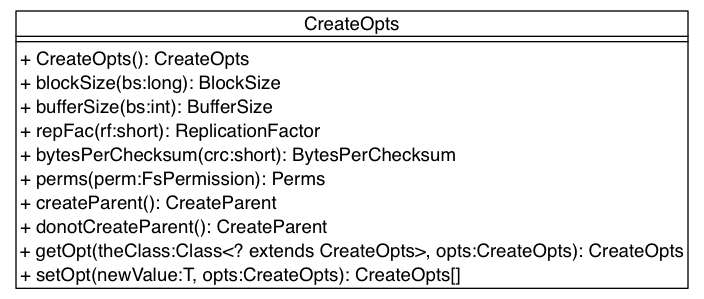
\includegraphics[width=10cm]{cdig/CreateOpts.png}
         
 静态内部类CreateOpts支持create方法中实现可变参数

        \begin{XeMethod}{\XeProtected}{CreateOpts}{getOpt}
             
 从想要的数据类型中获得option
 当option为null则抛出IllegalArgumentException("Null opt")异常

        \end{XeMethod}

        \begin{XeMethod}{\XeProtected}{CreateOpts[]}{setOpt}
             
 对指定的option设置或更新一个新的值newValue

        \end{XeMethod}

        \begin{XeInnerClass}{BlockSize}
\includegraphics[width=10cm]{cdig/BlockSize.png}
             
 BlockSize内部类继承自CreateOpts类
 内部含有blockSize常量

        \end{XeInnerClass}
        \begin{XeInnerClass}{ReplicationFactor}
\includegraphics[width=10cm]{cdig/ReplicationFactor.png}
             
 ReplicationFactor内部类继承自CreateOpts类
 内部含有replication常量

        \end{XeInnerClass}
        \begin{XeInnerClass}{BufferSize}
\includegraphics[width=10cm]{cdig/BufferSize.png}
             
 BufferSize内部类继承自CreateOpts类
 内部含有bufferSize常量

        \end{XeInnerClass}
        \begin{XeInnerClass}{BytesPerChecksum}
\includegraphics[width=10cm]{cdig/BytesPerChecksum.png}
             
 BytesPerChecksum内部类继承自CreateOpts类
 内部含有bytesPerChecksum常量

        \end{XeInnerClass}
        \begin{XeInnerClass}{Perms}
\includegraphics[width=10cm]{cdig/Perms.png}
             
 Perms内部类继承自CreateOpts类
 内部含有permissions常量

        \end{XeInnerClass}
        \begin{XeInnerClass}{Progress}
\includegraphics[width=10cm]{cdig/Progress.png}
             
 Progress内部类继承自CreateOpts类
 内部含有progress常量

        \end{XeInnerClass}
        \begin{XeInnerClass}{CreateParent}
\includegraphics[width=10cm]{cdig/CreateParent.png}
             
 CreateParent内部类继承自CreateOpts类
 内部含有createParent常量

        \end{XeInnerClass}
    \end{XeInnerClass}
\end{XeClass}
